\documentclass[a4paper,10pt,twocolumn,uplatex]{jsarticle}
\usepackage{style/nislab,style/resume}

%---------------------------------------------------------------------
% レジュメ種別・日付設定(要変更)
% \type{} 1:修士論文諮問会 2:卒業論文発表会 3:月例発表会 4:研究室合同発表会
%---------------------------------------------------------------------
\type{3}
\year{2021}
\month{4}
\date{1}

%---------------------------------------------------------------------
% ページ番号設定(要変更)
%---------------------------------------------------------------------
\setcounter{page}{1}

%---------------------------------------------------------------------
% 変更不要
%---------------------------------------------------------------------
\begin{document}

%---------------------------------------------------------------------
% タイトル作成部分(要変更)
% \maketitle{タイトル}{title}{名前}{name}
%---------------------------------------------------------------------
\maketitle{タイトルタイトルタイトルタイトルタイトルタイトル}
{Title Title Title Title Title Title}
{研究 太郎}
{Taro Research}

%---------------------------------------------------------------------
\section{はじめに}
大学でもっとも重要なのは論文・レポートを作成するということである.論文をきちんと書く能力を身につけずに社会に出ることは,大学卒の肩書きはあってもその能力に欠けているということを示すものに他ならない.というのも,論文を執筆すると言う作業は,自らの思考を論理的に構築し,それを他者(読者)に伝達する「プレゼンテーション能力」「コミュニケーション能力」そのものであり,多少,口先がうまいという程度ではなく,きちんとしたリサーチと分析・理解を踏まえた,論理的な思考の構築の過程を表現することが求められるからである.

%---------------------------------------------------------------------
\section{図表のベストプラクティス}
\LaTeX{}を使いこなすにあたり,図表の活用は重要である.基本的にはLaTex Wiki\cite{LaTexWiki}を参考にすれば問題ない.\par

%---------------------------------------------------------------------
\subsection{図}
図を挿入する場合は,図\ref{fig:sample1}や\figref{fig:sample2}のように引用することができる.図の横幅が大きい場合は,\figref{fig:sample2}のようにすることもできる.\par
ちなみに,\LaTeX{}ではベクターファイルとしてEPSファイルを推奨していた頃もあったようだが,現在はPDFファイルを使用することが推奨されている.PDFファイルに出力するのが前提なら,dvipdfmxではPDF,PNG,JPEG がそのまま使用できる.dvipdfmxはEPSファイルそのものを自分で扱えないので,Ghostscriptを内部で呼び出して変換する.PDFファイルで問題がなければEPSにこだわる必要はないと思われる.ただし,ジャーナルによっては図としてPDFを使うのがダメだったりするので慎重に.

\begin{figure}[!tb]
  \centering
  
\includegraphics[width=\linewidth]{img/sample1.pdf}
  \caption{悩む男の子}
  \label{fig:sample1}
\end{figure}

\begin{figure*}[!tb]
  \centering
  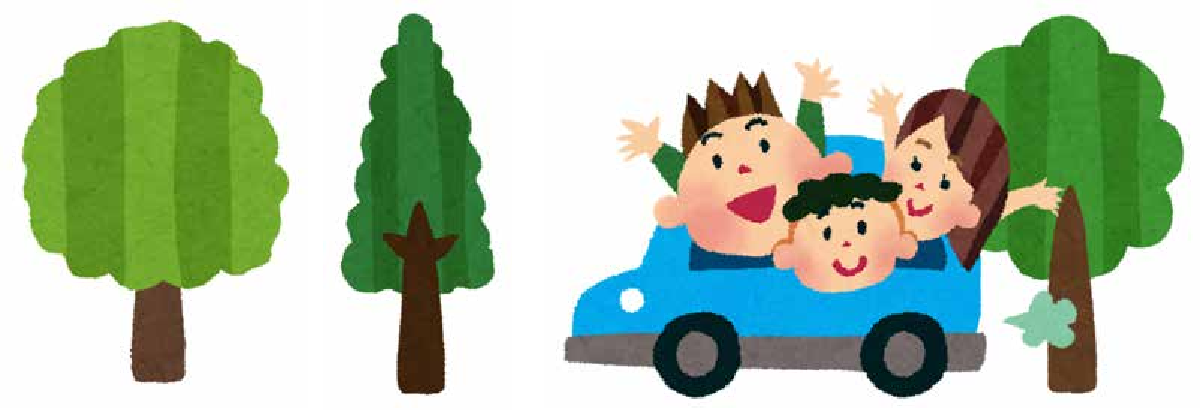
\includegraphics[width=\linewidth]{img/sample2.pdf}
  \caption{ドライブする家族}
  \label{fig:sample2}
\end{figure*}

%---------------------------------------------------------------------
\subsection{表}
表は\tabref{tab:data_type}のように引用することができ,表を作成する場合は罫線を少なくすることと,横線のみの使用を心がけることが推奨される.

\begin{table}[!bt]
  \caption{代表的なデータの型}
  \label{tab:data_type}
  \centering
  \begin{tabular}{lcr}
    \hline
    データの型         & 宣言   & ビット幅 \\
    \hline \hline
    短整数型           & short  & 16       \\
    整数型             & int    & 32       \\
    単精度浮動小数点型 & float  & 32       \\
    倍精度浮動小数店型 & double & 64       \\
    \hline
  \end{tabular}
\end{table}

%---------------------------------------------------------------------
\section{研究者にとっての論文十箇条}
論文を書くことは大切だ必要だ,と周囲から言われる.それは自分でも分かっているつもりだけれど,その理由をはっきりと伝えてもらえる機会は少ない.研究者にとっての論文十箇条\cite{渡辺豊2016}は,とてもシンプルでわかりやすく,非常に心にきた.一度目を通してみるべきであろう.

\begin{enumerate} % 箇条書きは \begin{itemize}
  \item 書かれた論文は書いた人の研究者としての人格を表す
  \item データのみ出して論文を書かない者は,テクニシャンである
  \item データも出さず,論文(原著論文)を書かない者は,評論家である
  \item 研究者は論文を書くことによって成長する.また,成長の糧にしなければならない
  \item 論文は研究者の飯のタネである
  \item 論文は後世の研究に影響を与えなければならない
  \item 研究者は書いた論文に責任を問われる
  \item 忙しくて論文が書けないというのは,言い訳にはならず,能力がないといっているのと同じである
  \item 博士論文以上の論文を書けない者は,その博士論文は指導教官のものといわれても仕方がない
  \item 研究において最も重要なのはアイデアであり,それが試されるのが論文である
\end{enumerate}

\section{おまけ}
おまけおまけおまけおまけおまけおまけおまけおまけおまけおまけおまけおまけおまけおまけおまけおまけおまけおまけおまけおまけおまけおまけおまけおまけおまけおまけおまけおまけおまけおまけおまけおまけ

%---------------------------------------------------------------------
% Bibliography(参考文献)
%---------------------------------------------------------------------
% thebibliography を利用する場合は以下を使用
\footnotesize{
  \begin{thebibliography}{99}
    \bibitem{LaTexWiki} Latex Wiki. \url{https://texwiki.texjp.org/}.
    \bibitem{渡辺豊2016} 渡辺 豊, "角皆静男先生のご逝去を悼む", 地球化学, vol.50, no.1, pp.1-3, 2016.
  \end{thebibliography}
}

% BibTex を利用する場合は以下を使用(初めての人には難しいかも)
% \bibliographystyle{junsrt}
% \bibliography{myref}

%---------------------------------------------------------------------
\end{document}
%---------------------------------------------------------------------
